\chapter{Preliminaries and Related Work}\label{preliminaries}

\section{Neighbors within Radius $r$}\label{flocking}

Bird flocking or distributed behavior model was first studied in~\cite{Reynolds1987} to animate the aggregate motion in computer simulation. An evaluation metric towards three aspects, separation, cohesion and alignment were also introduced. Based on this and observations,~\cite{Vicsek1995} has proposed a discrete-time model (\ref{eq:vicsek}) and discussed the relationship between the coherence of flocking and the density of particles. In this model, each particle has a constant velocity, while its direction is determined by ${\langle\theta(t)\rangle}_r$, which is the average direction of the neighboring particles within radius $r$, with $\Delta\theta$ representing the random noise.

\begin{equation}\label{eq:vicsek}
\begin{aligned}
x_i(t+\Delta t)&=x_i(t)+v_i(t)\Delta t\\
\theta(t+\Delta t)&={\langle\theta(t)\rangle}_r+\Delta\theta
\end{aligned}
\end{equation}

In natural flocking, however, the velocity of each bird is various that (\ref{eq:vicsek}) can not be simply applied. Nor the cohesion and collision avoidance criteria can be promised.~\cite{CuckerSmale2007} has proposed a control law for both discrete-time and continuous-time (\ref{eq:motion}, \ref{eq:cs_aij}, \ref{fig:cs_aij}) cases, where with given condition, the convergence of the flock to a common velocity is guaranteed. We identify the set of $N$ agents as $V=\{1,...,N\}$.

\begin{equation}\label{eq:motion}
\ddot{x}_i(t)=\underbrace{\sum^k_{j=1}a_{ij}(x)(v_j-v_i)}_{\text{velocity-consensus term}}+\underbrace{(-\bigtriangledown_{x_i}V_i)}_{\text{gradient-based term}}
\end{equation}

\noindent
$x_i, v_i$ and $u_i$ represent the position, velocity and input of agent $i$ at time $t$ respectively. Unless otherwise noted, we assume agents are at distinct positions, $x_i(0)\neq x_j(0)$ for $i, j\in V$. The weight function $a_{ij}:\mathbb{E}^k\to[0,\infty)$ qualifies the influence of agent $j$ on agent $i$, which is a function of agents' positions. In~\cite{Vicsek1995}, $a_{ij}$ is equally defined as (\ref{eq:vicsek_aij}), an example of $a_{ij}$ is illustrated in Fig.~\ref{fig:v_aij}.

\begin{equation}\label{eq:vicsek_aij}
a_{ij}(x)=\left\{\begin{array}{rcl}
1, & & \text{if $||x_i-x_j||\leq$ r}\\
0, & & \text{otherwise}
\end{array} \right.
\end{equation}

\begin{equation}\label{eq:cs_aij}
a_{ij}(x)=\frac{K}{(\sigma^2+||x_i-x_j||^2)^{\beta}}
\end{equation}

\begin{figure}[htb]
  \centering
  \subfigure[$a_{ij}(x)$ with $R=1$ in~\cite{Vicsek1995}]{\label{fig:v_aij}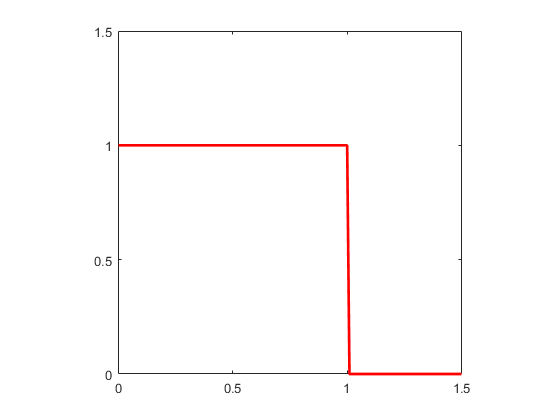
\includegraphics[width=0.32\textwidth]{figure/chapter_2/vicsek_aij.png}}
  \subfigure[$a_{ij}(x)$ with $\sigma=1$, $K=1$ and $\beta=0.5$ in~\cite{CuckerSmale2007}]{\label{fig:cs_aij}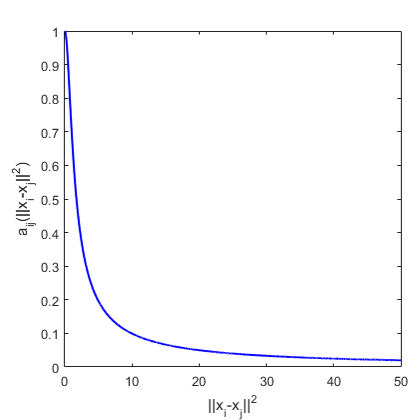
\includegraphics[width=0.32\textwidth]{figure/chapter_2/cs_aij.png}}
  \subfigure[$f(x)$ with $d_0=1$ and $\theta=1.2$ in ~\cite{CuckerDong2010}]{\label{fig:dong_f}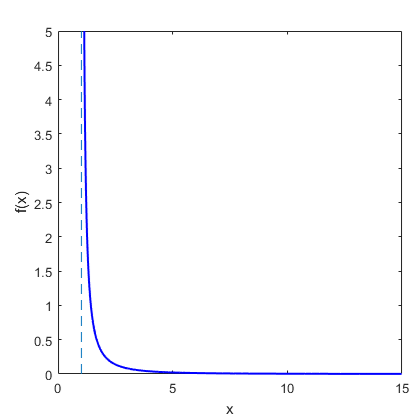
\includegraphics[width=0.32\textwidth]{figure/chapter_2/dong_f.png}}
  \caption{Examples of $a_{ij}(x)$ in~\cite{Vicsek1995},~\cite{CuckerSmale2007} and $f(x)$ in~\cite{CuckerDong2010}}\label{fig:example_v}
\end{figure}

Based on~\cite{CuckerSmale2007},~\cite{CuckerDong2010} has further proved the cohesion and separation of the flocks given $\beta\leq\frac{1}{2}$, by appending a collision avoidance term to the $u_i(t)$ in (\ref{eq:motion}), as shown in (\ref{eq:dong_aij}). The definition of $a_{ij}$ remains the same as (\ref{eq:cs_aij}). Where $f:(d_0,\infty)\to[0,\infty)$ is any repelling function satisfying: for any $d>d_0$, $\int_{d_0}^d f(x)dx=\infty$ and $\int_d^{\infty} f(x)dx<\infty$. An example $f(x)=\frac{1}{(x-d_0)^{\theta}}$ is illustrated in Fig.~\ref{fig:dong_f}.

\begin{equation}\label{eq:dong_aij}
\begin{aligned}
\ddot{x}_i(t)&=\sum^k_{j=1}a_{ij}(x)(v_j-v_i)+\underbrace{\Lambda(v)\sum_{j\neq i}f(||x_i-x_j||^2)(x_i-x_j)}_{\text{collision-avoidance term}}\\
\Lambda(v)&=(\frac{1}{k}\sum_{i>j}||v_i-v_j||^2)^{\frac{1}{2}}
\end{aligned}
\end{equation}

In~\cite{Saber2004}, the author claims the proposed model (\ref{eq:saber}) embodies all three flocking rules from~\cite{Reynolds1987}, where $\phi(\cdot)$ is a potential function, $n_{ij}$ is a vector along the line connecting $x_i$ and $x_j$ and $a_{ij}$ denotes corresponding adjacency matrix. When the number of agents is greater than ten, however, fragmentation may occur that a collective navigational feedback pair $(x_r, v_r)$ has to be introduced.

\begin{equation}\label{eq:saber}
\ddot{x}_i(t)=\underbrace{\sum_{j\in V}a_{ij}(x)(v_j-v_i)}_{\text{consensus term}}+\underbrace{\sum_{j\in V}\phi(||x_j-x_i||_{\sigma})n_{ij}}_{\text{gradient-based term}}+\underbrace{(-c_1(x_i-x_r)-c_2(v_i-v_r))}_{\text{navigational feedback term}}
\end{equation}

\section{$K$ Nearest Neighbors}

Unlike above mentioned theories assume, \cite{PNAS} discovered that interaction between agents in flocking does not depend on the metric distance but rather on the topological distance. An average number of six to seven neighbors are involved in the interaction instead of neighbors within a fixed distance. An example is illustrated in Fig.~\ref{fig:knn}, when $q=3$, three closest neighbors of agent 1 and agent 5 are agents 2, 3 and 6 and agents 1, 4 and 6 respectively. Given conditioned initial starting position, velocity and original $a_{ij}$ in (\ref{eq:vicsek_aij}),~\cite{KNN} has proved the alignment of the velocity in flocks.

\begin{figure}[htb]
  \centering
  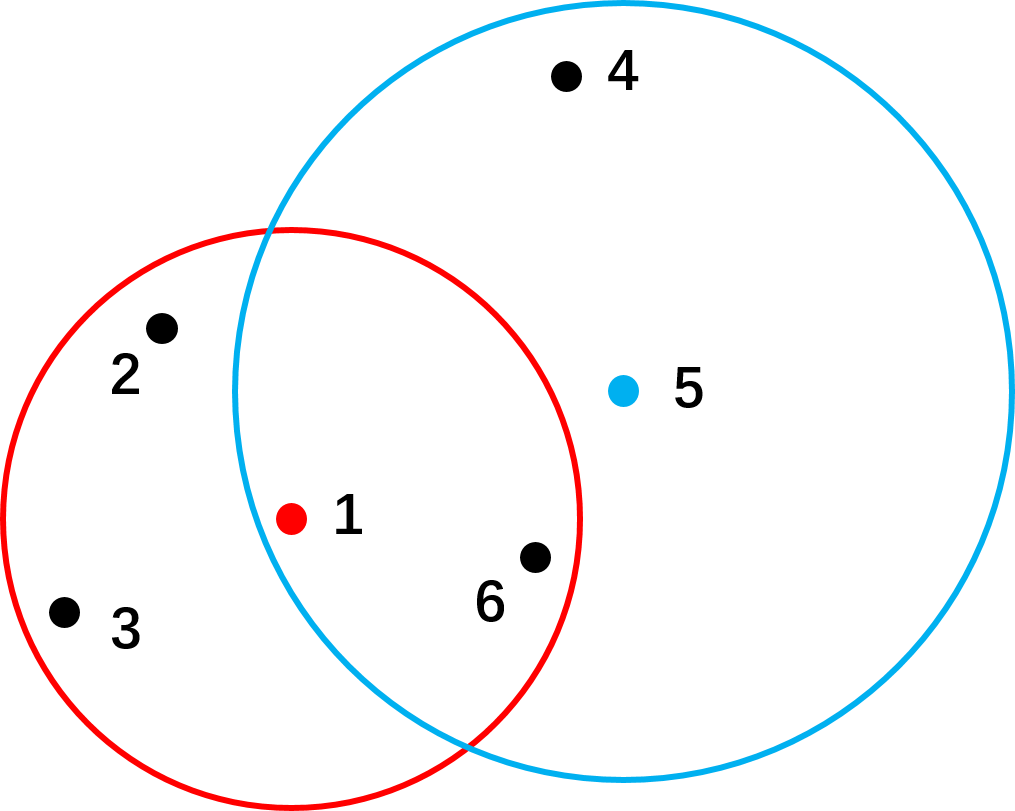
\includegraphics[width=0.5\textwidth]{figure/chapter_2/knn.png}
  \caption{A flock of six agents with $q=3$}
  \label{fig:knn}
\end{figure}

\noindent
Based on~\cite{KNN},~\cite{CuckerDong2016} have further introduced the quotient $\frac{q}{k-1}$ that unconditional flocking occurs when $\frac{q}{k-1}\geq\frac{1}{2}$.

\newpage
